\documentclass[tikz]{standalone}
\usetikzlibrary{calc}

\begin{document}

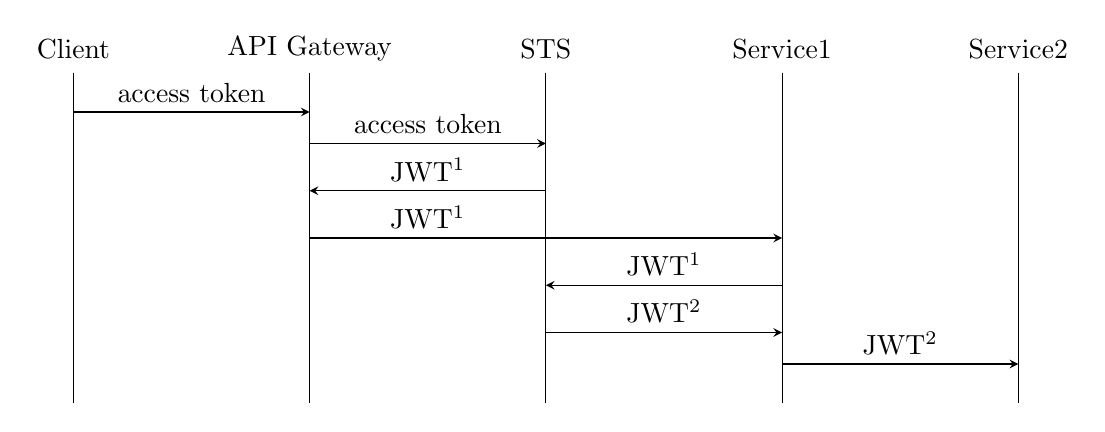
\begin{tikzpicture}
	\draw (-3,0) -- (-3,-4.2);
	\draw (0,0) -- (0,-4.2);
	\draw (3,0) -- (3,-4.2);
	\draw (6,0) -- (6,-4.2);
	\draw (9,0) -- (9,-4.2);
	\node at (-3,.3) {Client};
	\node at (0,.3) {API Gateway};
	\node at (3,.3) {STS};
	\node at (6,.3) {Service1};
	\node at (9,.3) {Service2};

	\draw[-stealth] (-3, -0.5) -- node[midway, above] {access token} (0, -0.5);
	\draw[-stealth] (0, -0.9) -- node[midway, above] {access token} (3, -0.9);
	\draw[-stealth] (3, -1.5) -- node[midway, above] {JWT\textsuperscript{1}} (0, -1.5);
	\draw[-stealth] (0, -2.1) -- node[pos = .35, above left] {JWT\textsuperscript{1}} (6, -2.1);
	\draw[-stealth] (6, -2.7) -- node[midway, above] {JWT\textsuperscript{1}} (3, -2.7);
	\draw[-stealth] (3, -3.3) -- node[midway, above] {JWT\textsuperscript{2}} (6, -3.3);
	\draw[-stealth] (6, -3.7) -- node[midway, above] {JWT\textsuperscript{2}} (9, -3.7);
	%\node[above,font=\large\bfseries] at (current bounding box.north) {Generate JWT for each request};
\end{tikzpicture}

\end{document}

